\documentclass[12pt]{article}

\usepackage[margin=1in]{geometry}

\usepackage{graphicx}
\usepackage{amsmath, amssymb, amsthm}
\usepackage{styles/stmaryrd}
\usepackage{styles/bussproofs}

\newcommand{\seq}[3]{#1:#2\longrightarrow#3}
\newcommand{\ignore}[1]{}

\begin{document}
\section{A Logic for Reasoning about Derivations in LF}
\begin{figure}
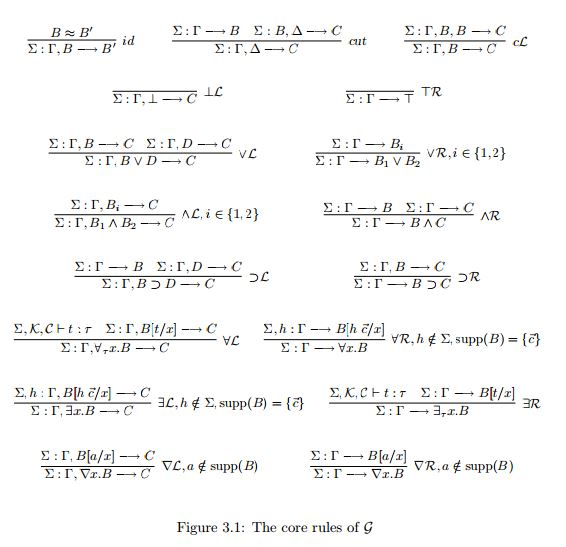
\includegraphics{Figure3-1.JPG}
\caption{Core Rules for $\mathcal{G}$ (From Andrew's Thesis)}\label{fig:metalogicG}
\end{figure}

\begin{figure}
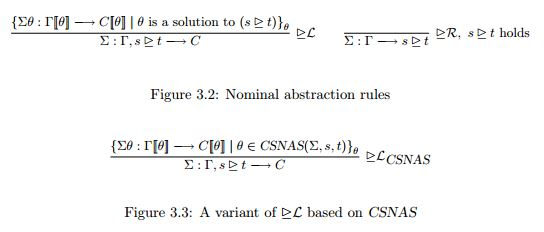
\includegraphics{Figure3-3.JPG}
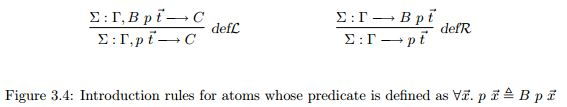
\includegraphics{Figure3-4.JPG}
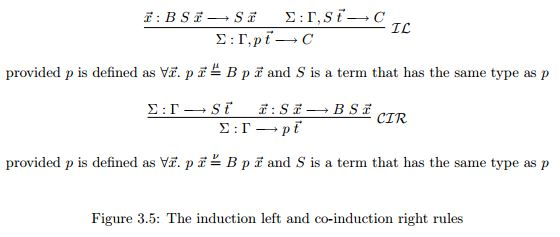
\includegraphics{Figure3-5.JPG}
\caption{Additonal Rules for $\mathcal{G}$ (From Andrew's Thesis)}\label{fig:metalogicG2}
\end{figure}

\begin{figure}
{\tt
Kind lftm type.\\
Kind lftp type.\\

Type lflam lftp -> (lftm -> lftm) -> lftm.\\
Type lfapp lftm -> lftm -> lftm.\\
Type lfpi lftp -> (lftm -> lftp) -> lftp.\\

Type of lftm -> lftp -> o.\\

Define hastype : olist -> lftm -> lftp -> prop by\\
  hastype G X A := member (of X A) G\\
; hastype G (lfapp M N) A := \\ 
      exists A1 A2, hastype G M (lfpi A1 A2) $\wedge$ hastype G N A1 $\wedge$ (A2 N) = A\\
; hastype G (lflam A M) (lfpi A B) := \\
      nabla x, hastype (of x A :: G) (M x) (B x).
}
\caption{Example Encoding of LF Typing Derivations}\label{fig:LFdef}
\end{figure}

The logic that I wish to use for reasoning is, at its core, the meta-logic $\mathcal{G}$.
%
Following the ideas of the 2-level-logic approach we extend the core logic with an encoding
of LF in $\mathcal{G}$ so that LF derivations are atomic formulas in the logic.
%
Figures~\ref{fig:metalogicG} and~\ref{fig:metalogicG2} show the derivation rules 
for $\mathcal{G}$.
%
The definition of LF in $\mathcal{G}$ should be given inductively so that case 
analysis on a derivation can be captured by the induction left rule. 
%
I will not right now present a complete definition of LF in $\mathcal{G}$ but 
Figure~\ref{fig:LFdef} contains an example of how one might encode LF typing 
judgments for object-level terms in the logic.
%
For now, let us suppose an adequate encoding exists and the notation for LF 
derivations is $\{\Gamma\vdash U : P\}$.
%
We would like to show that this logic is at least as expressive as $\mathcal{M}_2$ 
for reasoning about LF derivations.

\section{The Meta-Logic $\mathcal{M}_2$}


\section{Translating $\mathcal{M}_2+$ Theorems}
\ignore{
A theorem in $\mathcal{M}_2+$ consists of a context schema along with a formula.
%
A context schema describes the regular extension of the world and consist of some 
number of blocks describing the various assumption sets which may be added dynamically.
%
Formulas are constructed from conjunctions, universals, existentials, 
quantification over blocks, and $\top$.
%
The syntax is summarized in the following table.

\begin{align*}
Context~Form \quad\quad & C~::=~\cdot ~|~C,x:A\\
Block~Schema \quad\quad & B~::=~SOME~C_1.BLOCK~C_2\\
Context~Schema \quad\quad& S~::=~\cdot ~|~S,B\\
&\\
General~Formulas \quad\quad& G~::=~\square S.F\\
Formulas \quad\quad& F~::=~\forall x:A.F~|~\Pi p.F~|~\exists x:A.F~|~F_1\wedge F_2~|~\top\\
\end{align*}

Given a theorem written in this form we can transform it in two general chunks: 
first the context schema is used to construct a context definition in the logic
$\mathcal{G}$, and second the formula is translated using this newly defined 
context predicate.
%
The general idea behind the context definition is to construct a case for each 
block schema.

The translation for a single block schema, $\rho$, is given by
\begin{gather*}
\rho(SOME~x_1:A_1,\ldots ,x_n:A_n.BLOCK~y_1:B_1,\ldots ,y_m:B_m)=\\
nabla~y_1 \ldots y_n,~ctx~(\{y_m:B_m\} :: \ldots :: \{y_1:B_1\} :: G)~:=~\\
ctx~G \wedge \{G\vdash x_1:A_1\}~\wedge\ldots\wedge \{G\vdash x_n:A_n\}
\end{gather*}
%
By explicitly including the type restrictions for $x_1,\ldots,x_n$ in the clause 
we ensure that only well formed judgments are allowed in a context.
%
Once all of the block schemas are translated they are collected together as the 
context definition.

Now we will turn to the translation of formulas, $\phi$.
%
The translated formula always begins with capturing the context schema for the 
formula using the context definition.
%
Because of this we write $\phi_G$ to indicate that we are translating under the 
LF context G; so the translation of a formula $F$ becomes 
$\forall G,~ctx~G\rightarrow\phi_G(F)$.
%
This $G$ is used in the rest of the translation for the formula to index 
derivations by the context under which they hold.
%
Let us consider the quantifiers $\forall$ and $\exists$; the type restriction 
placed on the variable being quantified is extracted as an LF derivation in the 
following way
\begin{align*}
\phi_G(\forall x:A.F) &= forall~x, \{G\vdash x:A\}\rightarrow \phi_G(F)\\
\phi_G(\exists x:A.F) &= exists~x, \{G\vdash x:A\}\rightarrow \phi_G(F)
\end{align*}
%
The quantification over blocks is a bit more complex; essentially they quantify 
over a list of variables which correspond to one of the block schemas defined as 
part of the contex schema.
%
I interpret these as stating "for any subsequence of the context matching this form...", 
but this is a weak understanding based on a single example usage from Carsten's thesis.
%
When translating this quantifier we use nabla to introduce fresh variables for each
parameter variable and extend the context with these typing declarations in 
translating the remaining formula.
%
\begin{align*}
\phi_G(\Pi (y_1:B_1,\ldots,y_m:B_m).F) &= 
  nabla~y_1\ldots y_m, \phi_{G,\{y_1:B_1\},\ldots,\{y_:B_m\} }(F)
\end{align*}
%
The remaining two cases are straightforward; translating a conjunction is the 
conjunction of the translated components, and $\top$ is left unmodified.
\begin{align*}
\phi_G(F_1\wedge F_2) &= \phi_G(F_1)\wedge\phi_G(F_2)\\
\phi_G(\top) &= \top
\end{align*}

Once the statement has been translated we can turn to considering how an understanding
of the proof in $\mathcal{M}_2+$ can drive the construction of a proof for the 
translated theorem.
%
To begin this discussion we can consider an extension of the translation given above 
to the provability judgment for $\mathcal{M}_2+$, $\Psi;\Delta\vdash F$.
%
On the left-hand side of $\vdash$ are $\Psi$, the LF context, and $\Delta$, a 
list of the meta-assumption formulas, and on the right-hand side is $F$, the 
formula to be shown.
%
To translate this into a sequent $\Sigma;\Gamma\rightarrow G$ we first construct 
the signature $\Sigma$ from the variable names used in $\Psi$.
%
The $\Gamma$ is constructed starting from the assumption $ctx G$ and then 
collecting all the typing information, $x:A$, given in $\Psi$ and generating 
the assumptions $\{G|-x:A\}$ for each.
%
If a parameter variable is reached in $\Phi$ then the context $G$ used in the 
LF judgments is extended to include the additional block.
%
Finally, the translation of each formula in $\Delta$ is added to $\Gamma$ as 
an assumption.
%
The formula to be shown, $F$, and simply be translated using $\phi$ into the 
goal formula of our sequent.

Under this interpretation of the sequents, the rules of both systems are quite
similar, and so the understanding of the $\mathcal{M}_2+$ proof will translate 
into an understanding of the proof for our translated formula.
}
\end{document}
